\chapter{Инструменты для работы с Puppet}

\section{Подсветка синтаксиса для Vim}

Если вы любите программировать в консоли, то первым делом вам понадобится нормальная подсветка синтаксиса манифестов Puppet. Плагин VIM с её поддержкой можно взять с GitHub отсюда \url{https://github.com/puppetlabs/puppet-syntax-vim}. Просто скачайте репозиторий и скопируйте его содержимое в каталог ~/.vim.

В Ubuntu поддержку синтаксиса Puppet можно установить из репозитория

\begin{verbatim}
sudo aptitude install vim-puppet
\end{verbatim}

После чего включаем установленный плагин при помощи \textbf{vim-addon-manager}.

\begin{verbatim}
vim-addon-manager install puppet
\end{verbatim}

После этого vim должен показывать файлы \textbf{*.pp} с нормальной подсветкой синтаксиса.

\section{Проверка синтаксиса манифестов Puppet}

Чтобы проверить Puppet манифест на наличие синтаксических ошибок можно использовать \textbf{puppet parser validate}.

\begin{verbatim}
puppet parser validate manifest.pp
\end{verbatim}

Для проверки синтаксиса в шаблонах *.erb можно использовать такую команду 

\begin{verbatim}
erb -P -x -T '-' mytemplate.erb | ruby -c
\end{verbatim}

\section{Проверка на соответствие стандарту стили программирования Puppet манифестов}

Чтобы проверить не содержит ли модуль или манифест нарушений стандарта стиля кода Puppet (\url{http://docs.puppetlabs.com/guides/style_guide.html}), можно использовать утилиту \textbf{puppet-lint}.

Официальный сайт этой утилиты здесь \url{http://puppet-lint.com/}, а исходный код можно скачать с GitHub \url{https://github.com/rodjek/puppet-lint}.

Сначала установим gem.

\begin{verbatim}
gem install puppet-lint
\end{verbatim}

Теперь можно проверить все модули и увидеть список недостатков, которые желательно исправить.

\begin{verbatim}
> puppet-lint --with-filename /etc/puppet/modules
foo/manifests/bar.pp: trailing whitespace found on line 1
apache/manifests/server.pp: variable not enclosed in {} on line 56
...
\end{verbatim}

\section{Использование Vim как IDE для Puppet}

Если вы постоянно использует Vim для работы с манифестами Puppet и не хотите использовать полноценную среду разработки, то можно установить несколько плагинов, которые сделают из Vim легкий Puppet редактор.

\begin{figure}[h]
\centering
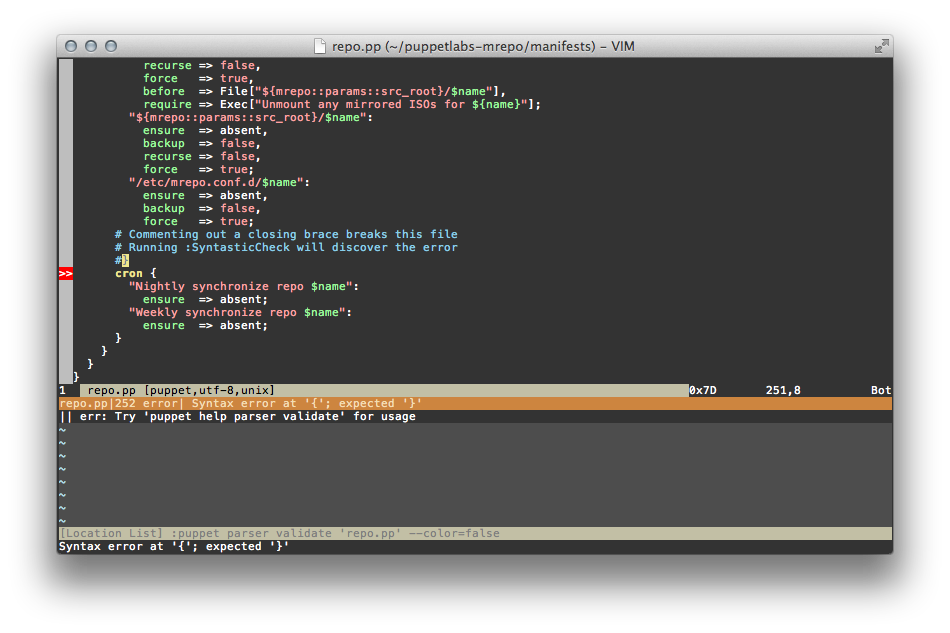
\includegraphics[width=0.8\textwidth]{img/syntastic.png}
\caption{Vim как IDE для Puppet}
\label{fig:syntastic}
\end{figure}

\begin{enumerate}
\item \url{https://github.com/rodjek/vim-puppet}
\item \url{https://github.com/scrooloose/syntastic}
\item \url{https://github.com/honza/vim-snippets}
\end{enumerate}

\section{Geppetto}

Geppetto --- продвинутая среда разработки для Puppet, созданная на основе Eclipse компанией \url{http://www.cloudsmith.com}. Предоставляет большинство функций, полезных для работы с Puppet.

\begin{itemize}
\item Подсветка синтаксиса манифестов
\item Автодополнение имен классов и функций
\item Автоматическая проверка на наличие синтаксических ошибок и ссылок на несуществующие объекты
\item Проверка на наличие стилистических ошибок и потенциальных проблем
\item Встроенная поддержка Git
\item Поддержка плагинов Eclipse, включая работу с rspec и интеграцию с Jenkins.
\end{itemize}

\begin{figure}[h]
\centering
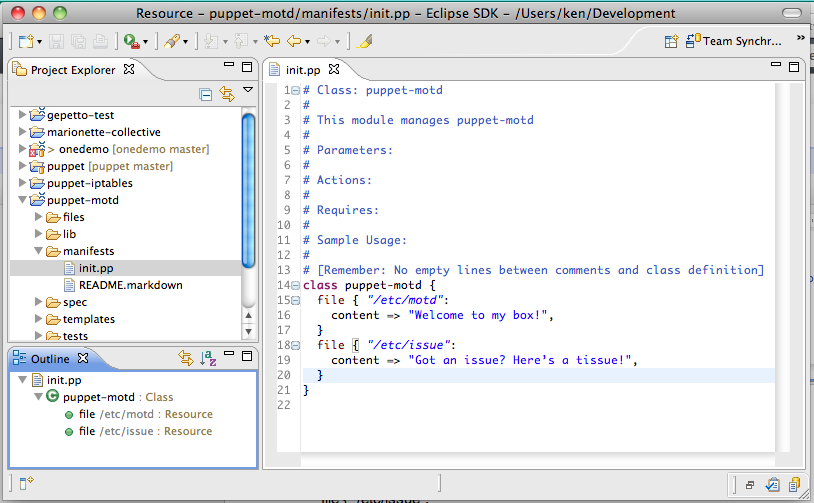
\includegraphics[width=0.8\textwidth]{img/geppetto.png}
\caption{Geppetto --- IDE для Puppet}
\label{fig:geppetto}
\end{figure}

\begin{description}
\item[Анонс на PuppetLabs] \url{https://puppetlabs.com/blog/geppetto-a-puppet-ide/}
\item[Страница на GitHub] \url{http://cloudsmith.github.io/geppetto/index.html}
\item[FAQ по Geppetto] \url{http://cloudsmith.github.io/geppetto/faq.html}
\item[Скачать Geppetto] \url{http://cloudsmith.github.io/geppetto/download.html}
\item[Видео демонстрация работы] \url{http://vimeo.com/21999983}
\end{description}
